\chapter{Firmware}

\hypertarget{ambiente-di-sviluppo}{%
\section{Ambiente di sviluppo}\label{ambiente-di-sviluppo}}

Come detto inizialmente, l'intero codice del progetto è \textit{open-source} ed è
visionabile al seguente link:\\
\href{https://github.com/thomasnonis/ppse-2021}{\underline{https://github.com/thomasnonis/ppse-2021}}.\\
Per lo sviluppo del codice abbiamo scelto di lavorare con l'ambiente
\emph{Microsoft Visual Studio Code}, in quanto molto versatile e
continuamente supportato dagli sviluppatori.\\
Per poter utilizzare le librerie del microcontrollore \emph{RP2040} è
stato necessario includere nel progetto il \emph{pico-sdk}, un kit di
sviluppo che permette di implementare le istruzioni \emph{HAL} (Hardware
Abstraction Level) per potersi interfacciare all'hardware del micro ed
alle sue relative periferiche. L'\emph{SDK} non è l'unica libreria a cui abbiamo fatto affidamento, infatti abbiamo aggiunto al progetto
anche \emph{pico-examples} e \emph{picotool}. Con \emph{pico-examples}
siamo riusciti a testare delle funzioni base del microcontrollore ed
allo stesso tempo a capire il processo di compilazione via
\emph{Makefile}, in quanto la libreria era dotata di molteplici esempi
base per ogni periferica offerta dal micro, mentre \emph{picotool} è
stata utilizzata per poter automatizzare il processo di flashing del
codice.\\
Le librerie citate appaiono nel progetto come \emph{submodules}, in
quanto, grazie al software di controllo versione \emph{git} è possibile
tenerle aggiornate senza che siano presenti vincoli legati a delle
specifiche versioni.

\hypertarget{compilazione}{%
\section{Compilazione}\label{compilazione}}

\noindent Durante una fase iniziale di testing abbiamo trovato delle difficoltà
per compilare il codice, in quanto nella documentazione ufficiale non
era ben chiaro come si dovessero scrivere e disporre in modo corretto i
file \textit{CMakeLists}. Con un po' di lavoro abbiamo deciso di strutturare la
compilazione nel seguente modo:

\begin{center}
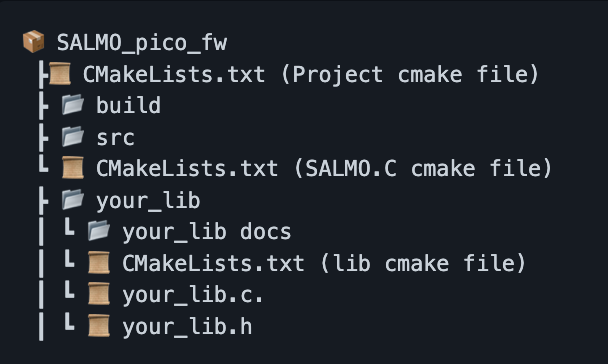
\includegraphics[width=0.4\textwidth]{figures/image73.png}
\captionsetup{type=figure}
\captionof{figure}{Struttura del codice di SALMO}
\end{center}

\noindent Ogni libreria contiene un proprio \textit{CMakeLists} in cui viene specificato il
nome della libreria (linkando i file .c e .h) e vengono \textit{linkate} altre librerie
esterne (come \emph{pico\_stdlib}).

\begin{center}
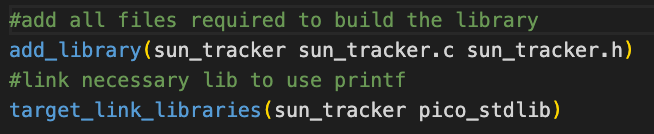
\includegraphics[width=0.7\textwidth]{figures/image45.png}
\captionsetup{type=figure}
\captionof{figure}{CMakeLists della libreria per il calcolo della posizione del sole}
\end{center}

\noindent Dopodichè nel main principale in cui verrà eseguito il codice (presente
in \emph{SALMO.c}), viene definito l'eseguibile (ovvero si linka il file
.c attribuendolo ad un nome), dopodiché si linkano le librerie definite
precedentemente e si includono anche le cartelle in cui queste sono
presenti, per poi opzionalmente decidere se abilitare altri parametri
come \emph{usb output} o \emph{uart output.}

\begin{center}
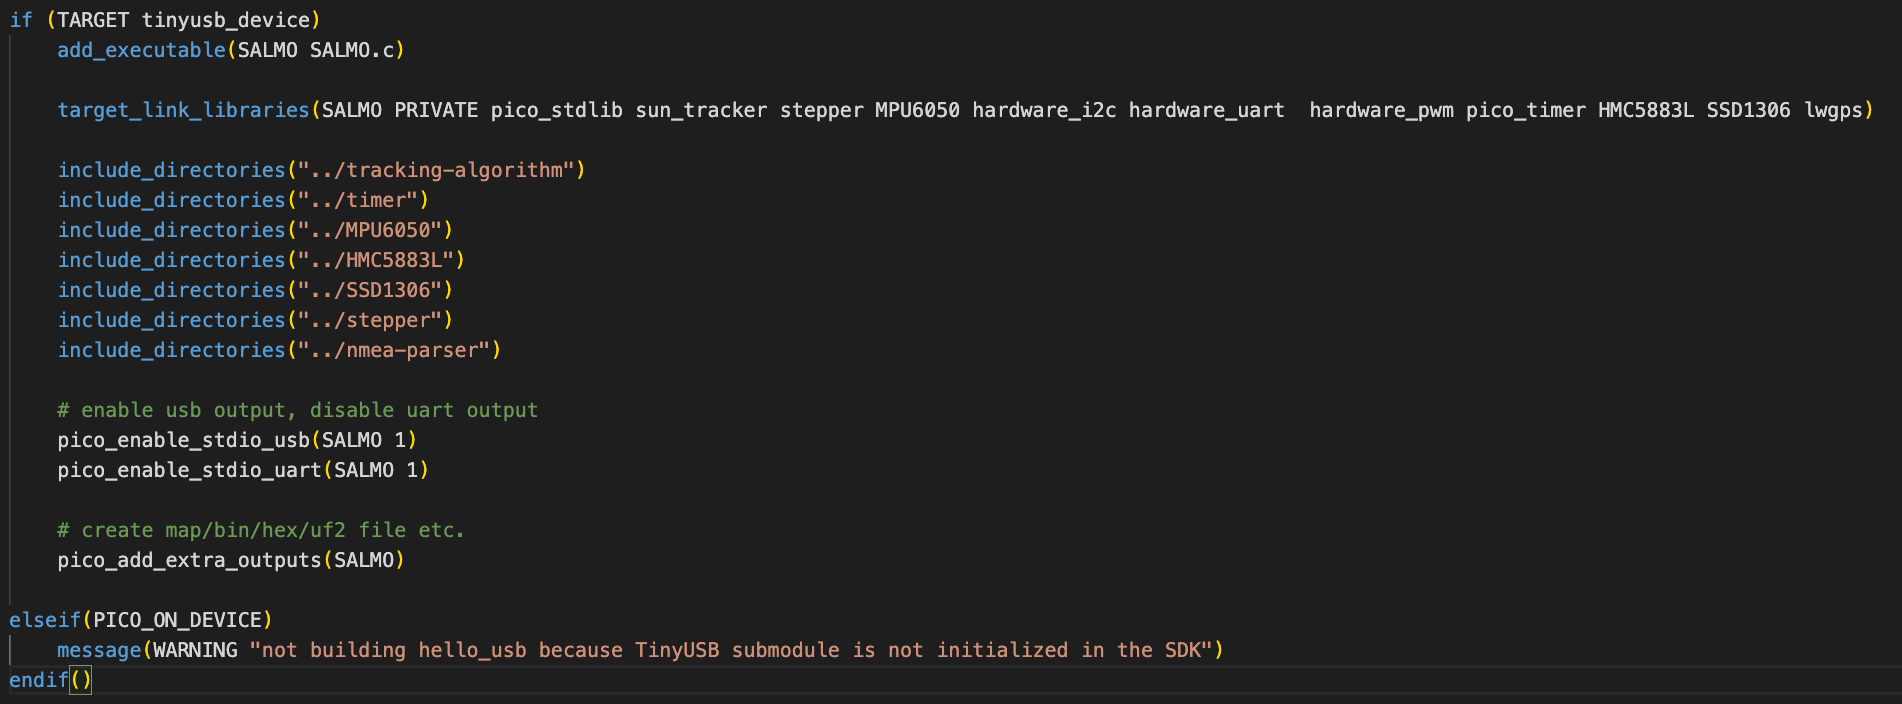
\includegraphics[scale=0.45]{figures/image66.png}
\captionsetup{type=figure}
\captionof{figure}{CMakeLists di SALMO.c}
\end{center}

\noindent I file \textit{CMakeLists} vengono ``eseguiti'' in ordine gerarchico, per cui è
necessario avere un \textit{CMakeLists} esterno che ha il compito di tenere
traccia di tutti gli altri \emph{CMakeLists} e di definire i parametri
relativi alla versione del \emph{CMAKE} e della versione del compilatore
C e C++. Per compilare il progetto SALMO è sufficiente quindi eseguire
il comando CMake sul file CMakeLists più esterno, producendo così un
Makefile che, una volta eseguito, compilerà autonomamente l'intero
progetto restituendo i file eseguibili necessari per flashare il
microcontrollore.

\begin{center}
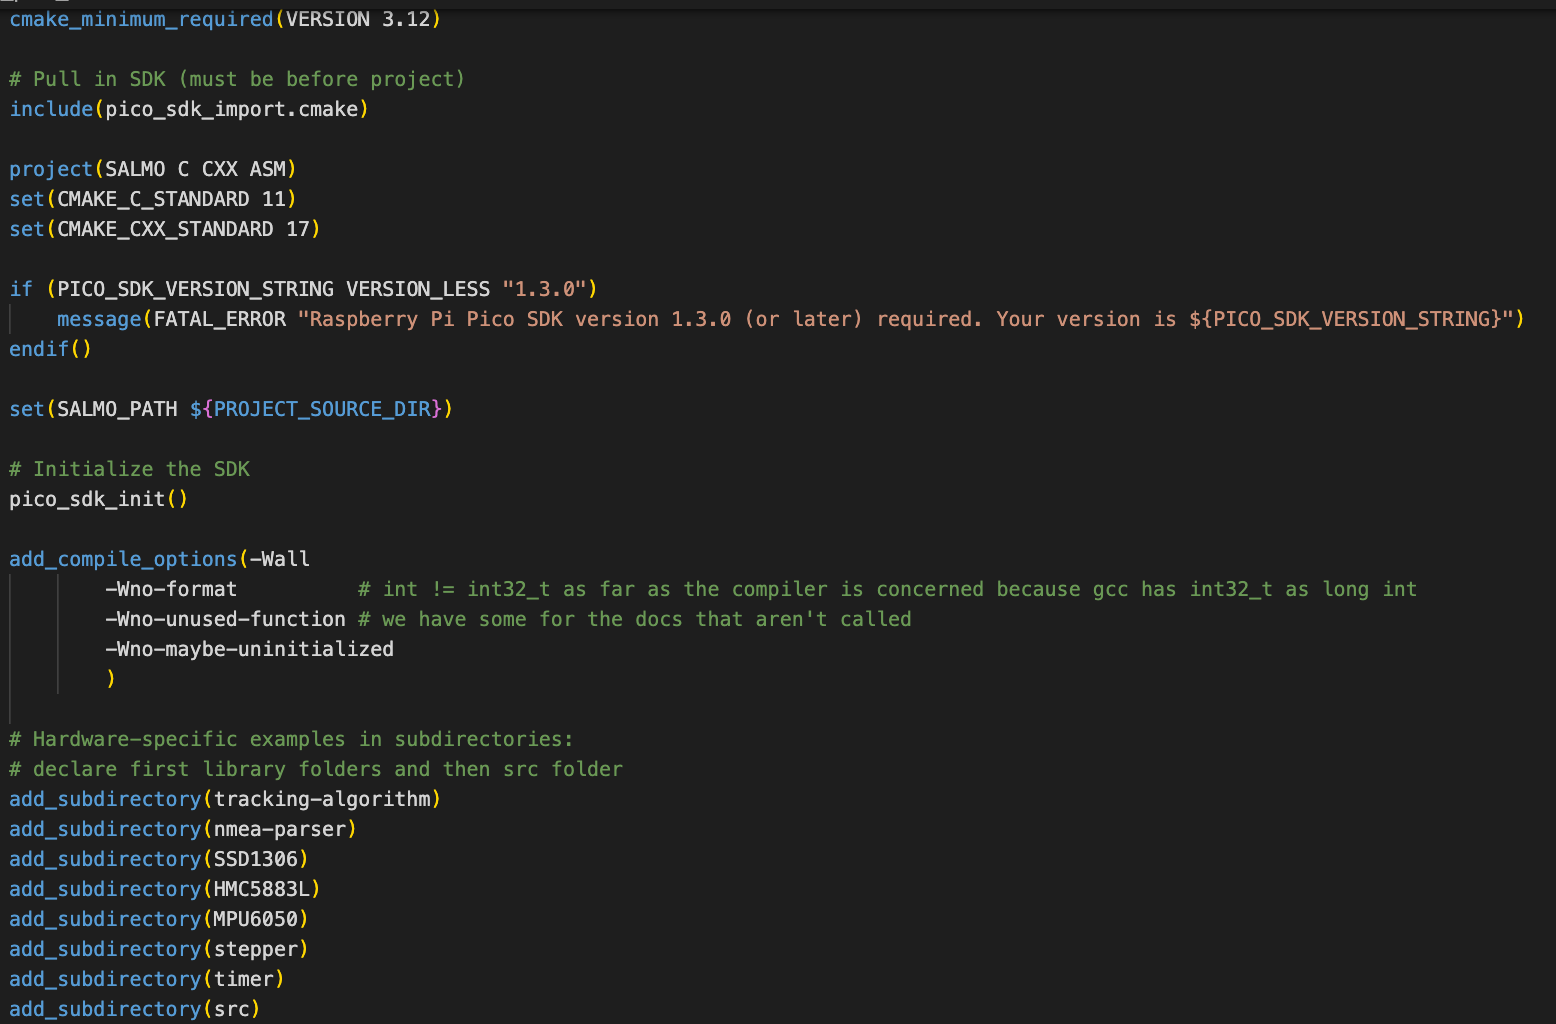
\includegraphics[scale=0.55]{figures/image67.png}
\captionsetup{type=figure}
\captionof{figure}{CMakeLists del progetto}
\end{center}

\noindent Per rendere più veloce la fase di compilazione abbiamo deciso di
scrivere tre piccoli script \emph{bash}, situati nella cartella
\emph{src}: \emph{build.sh}, \emph{flash.sh},
\emph{build\_and\_flash.sh}: lo script di build utilizza \emph{cmake}
per compilare i \emph{Makefile} e salvare i relativi eseguibili dentro
la cartella \emph{build}, mentre quello di flash utilizza
\emph{picotool} per caricare l'eseguibile in formato \emph{.uf2}
direttamente nella \emph{flash} del microcontrollore, anche se il \textit{RP2040}
non si trova in \textit{bootloader mode} (\emph{picotool} riavvia il MCU in
bootloader mode). Infatti se non usassimo \emph{picotool} dovremmo
resettare la scheda tenendo premuto il pulsante di boot per entrare in
bootloader mode, successivamente trascinare il file eseguibile
all'interno della partizione \textit{Mass Storage} del micro, per poi resettarlo
via pulsante. Lo script di \emph{build} è inoltre dotato di un
\emph{flag} opzionale attivabile scrivendo \emph{./build.sh all}, con il
quale viene rimossa l'intera directory di build ed il progetto viene
ricompilato da capo (utile in caso di errori del compilatore non
realmente presenti nel codice). Abbiamo scelto di flashare mediante
l'eseguibile con estensione \emph{.uf2} in quanto, utilizzando questo
tipo di file, è sufficiente copiare l'eseguibile nella partizione di
tipo \textit{Mass Storage} che il \textit{RP2040} offre una volta avviato in bootloader
mode.\\
Come intuibile, il file \emph{build\_and\_flash.sh} esegue sia le
operazioni di compilazione sia l'operazione di flashing.

\hypertarget{algoritmo-per-ottenere-la-posizione-del-sole}{%
\section{Algoritmo per ottenere la posizione del
sole}\label{algoritmo-per-ottenere-la-posizione-del-sole}}

\noindent Al fine di poter pilotare correttamente i motori verso il sole abbiamo
dovuto trovare un modo per convertire i dati ottenuti dal GPS in
elevazione ed azimuth del sole (espressi in gradi). Per approcciare
correttamente il problema abbiamo iniziato a leggere vari \emph{papers}
e relazioni tecniche riguardo ad algoritmi per la rilevazione della
posizione del sole, il primo, forse tra i più datati, è stato \emph{The
astronomical almanac's algorithm for approximate solar position} di
\emph{Joseph J. Michalsky}. Dopo alcune letture abbiamo capito che era
necessario passare tra vari sistemi di riferimento per ottenere le
coordinate del sole, in particolare ci siamo imbattuti nel concetto di
\emph{Julian Date} (giorni passati dalle 12 del 1 Gennaio 4713 B.C.),
coordinate celesti, \emph{GMST} (Greenwich Mean Sidereal Time, un giorno
siderale è 4 minuti più corto di un giorno solare) e \emph{LMST} (Local
Mean Sidereal Time). Nonostante nel paper di \emph{Michalsky} fosse
presente del codice \emph{FORTRAN} per l'implementazione dell'algoritmo,
non lo abbiamo ritenuto abbastanza ``solido'' ed efficiente per il
nostro tipo di applicazione.\\
Per poter verificare la corretta posizione del sole abbiamo utilizzato
questo sito come contro prova dei nostri calcoli:
\href{https://gml.noaa.gov/grad/solcalc/}{\underline{https://gml.noaa.gov/grad/solcalc/}}.

\begin{center}
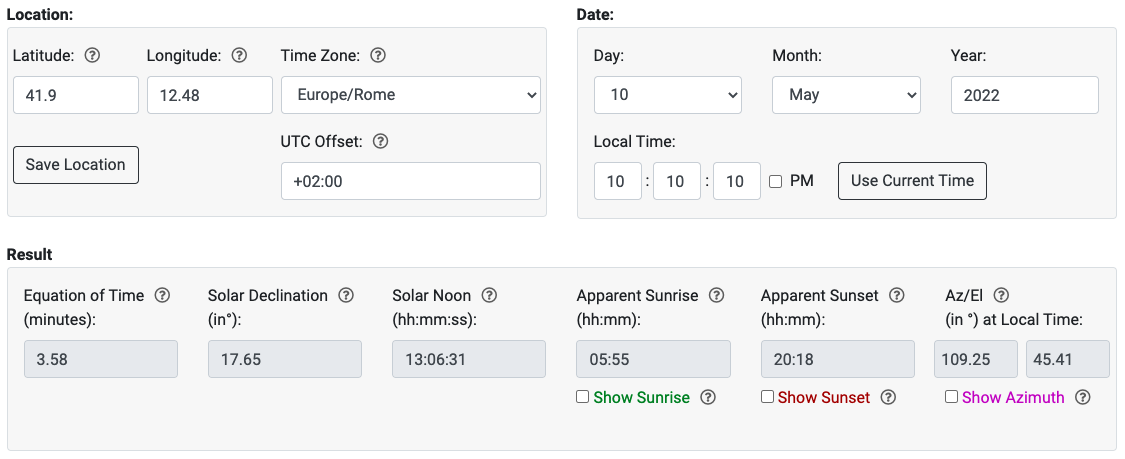
\includegraphics[scale=0.35]{figures/image72.png}
\captionsetup{type=figure}
\captionof{figure}{Interfaccia web NOAA solcalc}
\end{center}

\noindent Fortunatamente la \emph{NOAA} (National Oceanic and Atmospheric
Administration), oltre a fornire questa interfaccia web, condivide anche
i file \emph{excel} con cui vengono eseguiti i calcoli al fine di
ottenere gli stessi risultati presenti sul loro sito. Di conseguenza,
essendo questo \emph{tool} uno dei pochi affidabili in rete con cui
poter verificare i nostri calcoli, abbiamo deciso di riportare le
formule del file \emph{excel} in codice C per ottenere gli stessi
risultati. I calcoli intermedi non verranno riportati nel dettaglio in
quanto sono computazioni astronomiche che non rientrano nelle tematiche
trattate nel corso.\\
Per la computazione abbiamo fatto riferimento a due strutture dati, una
denominata \emph{Place} in cui viene salvata la data, l'orario e
latitudine e longitudine ``\emph{parsate}'' dal GPS (mediante una
libreria open source), e l'altra, \emph{Position,} in cui vengono
salvati tutti i parametri intermedi ed i risultati finali per il calcolo
della posizione del sole (basato sull'algoritmo della \emph{NOAA}).

\begin{center}
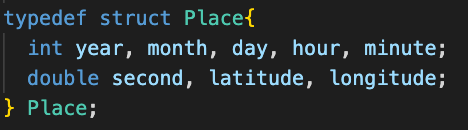
\includegraphics[scale=1]{figures/image25.png}
\captionsetup{type=figure}
\captionof{figure}{Struct "Place"}
\end{center}

\begin{center}
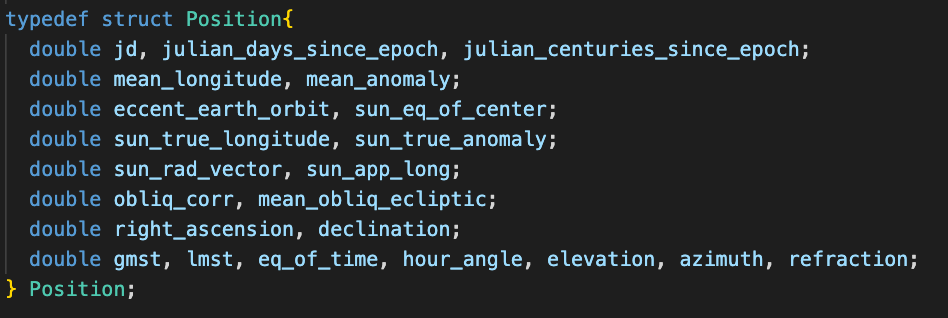
\includegraphics[scale=0.8]{figures/image33.png}
\captionsetup{type=figure}
\captionof{figure}{Struct "Position"}
\end{center}

\noindent Per calcolare la posizione esatta del sole infatti i dati contenuti in
\emph{Place} vengono utilizzati per ottenere una \emph{Julian Date},
una \emph{Julian Date} conteggiata a partire dalle 12 del primo Gennaio
2000 e successivamente tutti i parametri intermedi per poi ottenere
elevazione e azimuth del sole. In seguito ad alcuni test abbiamo
riscontrato che siamo in grado di ottenere un'ottima precisione,
addirittura nell'ordine del grado!

\hypertarget{implementazione-software-delle-periferiche}{%
\section{Implementazione software delle
periferiche}\label{implementazione-software-delle-periferiche}}

Tutte le periferiche, a meno di GPS, utilizzano interfaccia di
comunicazione \emph{I2C}.\\
Il protocollo hardware \emph{I2C} prevede due linee seriali di
comunicazione: \emph{SDA} (Serial DAta) per i dati e \emph{SCL} (Serial
CLock) per il clock (la comunicazione I2C è di tipo sincrono).\\
Siccome le linee \emph{SDA} ed \emph{SCL} sono di tipo Open-Drain (o
Open-Collector a seconda della tecnologia utilizzata) sono necessari dei
resistori di pull-up per portare a livello logico alto le linee. Nel
progetto \emph{SALMO}, siccome accelerometro e magnetometro vengono
acquistati sotto forma di moduli commerciali, troviamo già i resistori
di pull-up su di essi, per cui, questi ultimi, verranno dimensionati e
montati direttamente in solo uno dei moduli (verranno quindi rimossi
dagli altri).

\begin{center}
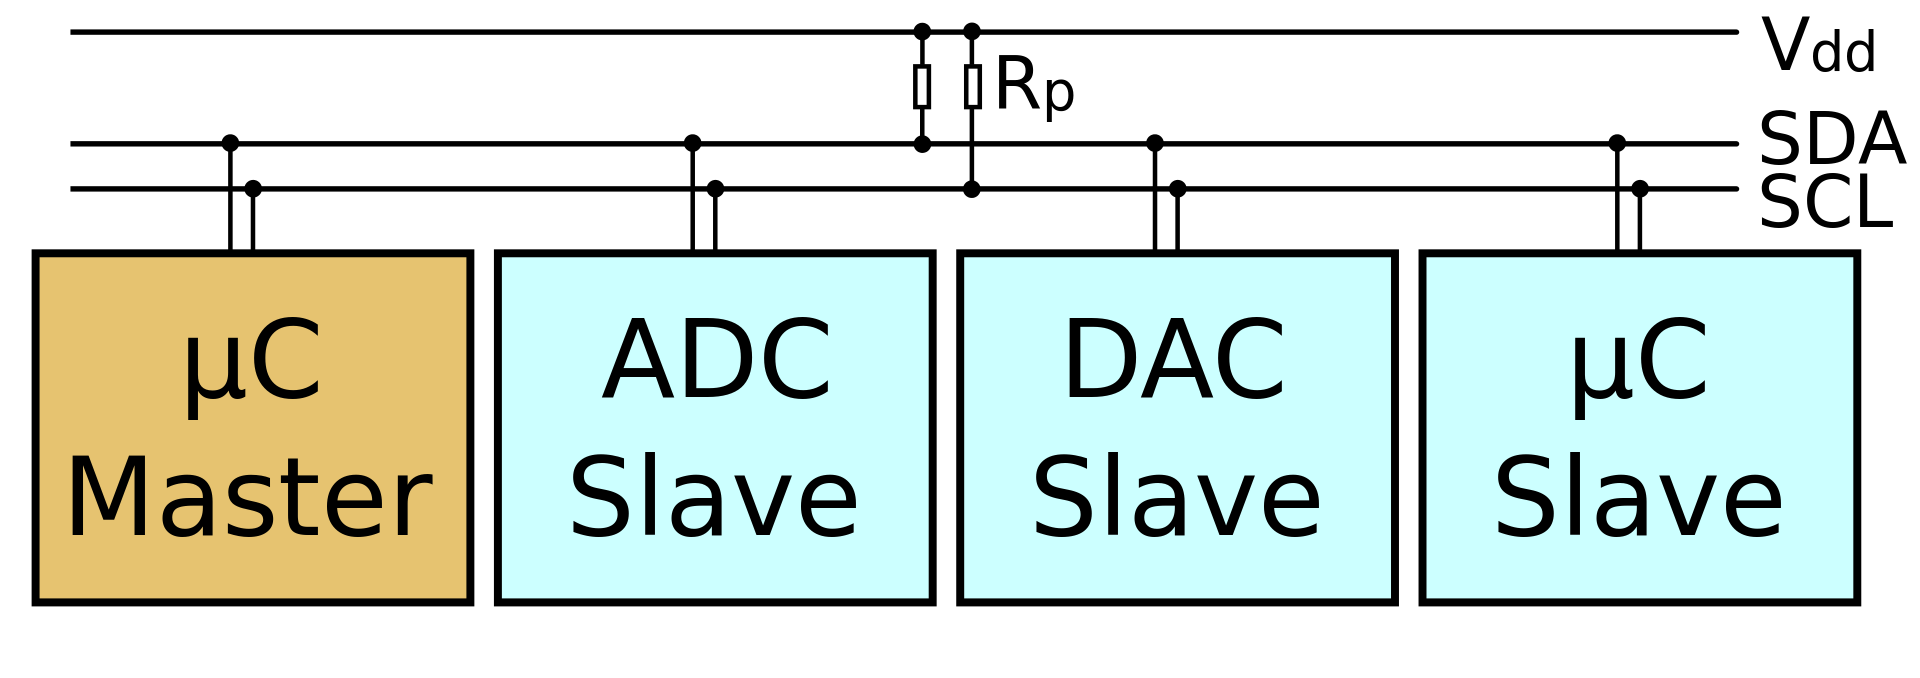
\includegraphics[width=0.5\textwidth]{figures/image61.png}
\captionsetup{type=figure}
\captionof{figure}{Esempio di bus I2C}
\end{center}

\noindent La struttura dei driver di HMC5883L e MPU6050 segue una logica ben
precisa, in modo da rendere particolarmente semplice e versatile il
codice:

\begin{itemize}
\item
  
  \textless drivername\textgreater\_defines.h
  
\item
  
  \textless drivername\textgreater\_I2C.h
  
\item
  
  \textless drivername\textgreater\_I2C.c
  
\item
  
  \textless drivername\textgreater.c
  
\item
  
  \textless drivername\textgreater.h
  
\end{itemize}

\noindent Utilizzando questa struttura è possibile innanzitutto separare tutte le
definizioni di registri ed indirizzi in un file header separato
(\textless drivername\textgreater\_defines.h) ed in secondo luogo, forse
vantaggio principale, è possibile dichiarare e definire le funzioni di
lettura e scrittura nel bus I2C in due soli file
(\textless drivername\textgreater\_I2C.h e
\textless drivername\textgreater\_I2C.c) in modo che il vero e proprio
driver (\textless drivername\textgreater.h e
\textless drivername\textgreater.c) rimanga completamente indipendente
dalle funzioni I2C. Questo, è particolarmente vantaggioso perché le
funzioni I2C sono dipendenti dal HAL offerto dall'SDK (e quindi in certo
senso dall'architettura), per cui nel caso in cui volessimo
ri-utilizzare i driver per un'altra architettura (es. STM32) sarebbe
sufficiente modificare solamente le due funzioni di lettura e scrittura
su bus I2C nel file \textless drivername\textgreater\_I2C.c .\\
Il microcontrollore offre due controller I2C: I2C0 ed I2C1. Nel progetto
SALMO viene utilizzato solo uno dei due controller, che viene condiviso
da accelerometro, magnetometro e display.\\
Tutte e 3 le periferiche utilizzano il bus in modalità fast, ovvero a
400KHz.\\
Per effettuare una lettura o la scrittura di un registro di una
periferica nel bus è necessario che il master invii un messaggio
specifico determinato dal protocollo I2C: bit di start, 7, 8 oppure 10
bit di indirizzo (HMC5883L utilizza 8 bit, mentre MPU6050 e SSD1306
utilizzano 7 bit di indirizzo), un bit che indica lettura o scrittura,
un bit di acknowledge da parte dello slave, e successivamente 8 bit di
dato (ad esempio il registro da leggere o il registro in cui si vuole
scrivere, seguito di nuovo da un bit di acknowledge. È possibile inviare
N blocchi da 8 bit seguiti dal bit di acknowledge dopo il bit di
read/write (anch'esso seguito da un bit di acknowledge).

\begin{center}
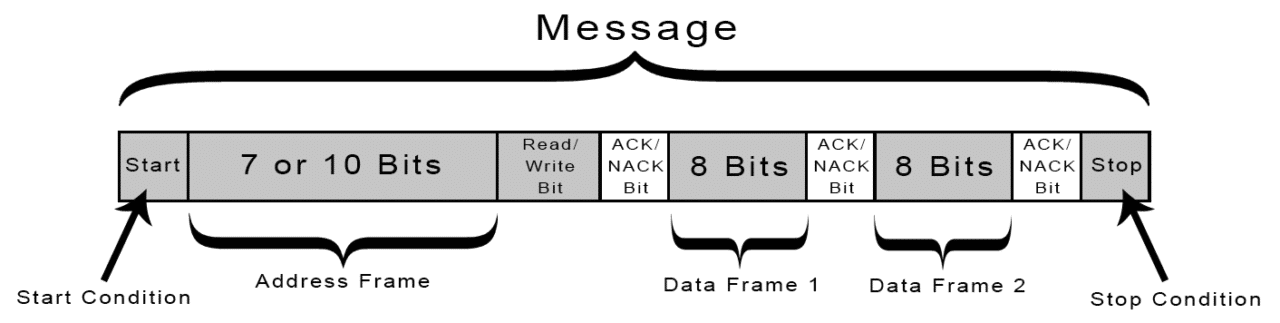
\includegraphics[scale=0.30]{figures/image51.png}
\captionsetup{type=figure}
\captionof{figure}{Data frame protocollo I2C}
\end{center}

\noindent Nel caso, ad esempio, in cui si voglia scrivere il contenuto di un
registro del MPU6050 è sufficiente inviare: bit di start, 7 bit di
indirizzo (LSB configurabile), bit di read (es. 0 1101000 1) che saranno
seguiti da un bit di acknowledge ed infine invieremo gli 8 bit
dell'indirizzo su cui vogliamo scrivere (es. 00111011). Successivamente
invieremo, dopo aver ricevuto l'acknowledge, i dati che vogliamo
scrivere.\\
Nel caso della lettura invece, è necessario ripetere la procedura
illustrata precedentemente fino all'invio dell'indirizzo del registro
(in questo caso da leggere) ed inviare un bit di start seguito
dall'indirizzo dello slave ed infine un bit di read. La periferica slave
invierà finalmente, sempre dopo il bit di acknowledge, il contenuto del
registro richiesto.

\begin{center}
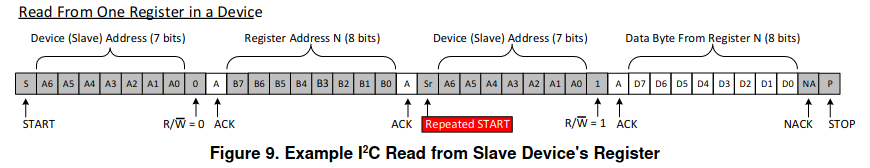
\includegraphics[scale=0.65]{figures/image39.png}
\captionsetup{type=figure}
\captionof{figure}{Data frame esempio lettura I2C}
\end{center}

\begin{center}
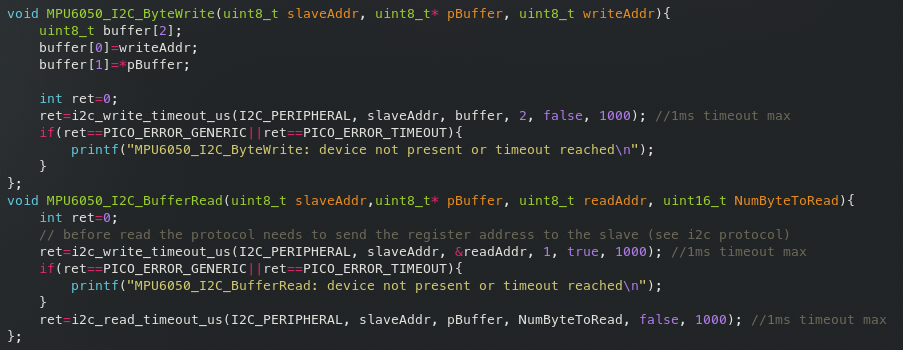
\includegraphics[scale=0.65]{figures/image35.png}
\captionsetup{type=figure}
\captionof{figure}{Funzioni di write e read I2C (driver MPU6050)}
\end{center}

\noindent Per quanto concerne l'implementazione software del display OLED, abbiamo
deciso di utilizzare la libreria già presente negli SDK di Raspberry
Pico (seppur per nulla completa). Sottolineiamo che attualmente il
driver di questa periferica non è stato completato poiché, non avendola
sotto mano, abbiamo deciso di prioritizzare il resto del lavoro.\\
Un altro protocollo di comunicazione utilizzato nel progetto è
\emph{UART} (\emph{Universal Asynchronous Receiver-Transmitter})che, come
visto nel primo modulo del corso, permette il trasferimento e ricezione
di dati in seriale ad un tasso di velocità [bit/s] fissato, detto baud
rate. Abbiamo inserito la configurazione \emph{UART} nel modulo
\emph{PAM7Q.c}, file in cui vengono inizializzati i pin RX e TX, e
vengono settati tutti i parametri necessari a comporre il data frame,
assumendo la seguente configurazione:

\begin{itemize}
\item
  
  Hardware flow: no
  
\item
  
  Baud rate: 9600 bit/s
  
\item
  
  Bit di dato: 8
  
\item
  
  Bit di stop: 1
  
\item
  
  Bit di parità: no
  
\end{itemize}

\begin{center}
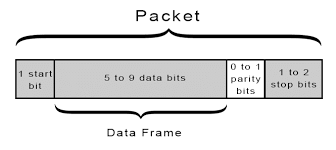
\includegraphics[width=0.4\textwidth]{figures/image46.png}
\captionsetup{type=figure}
\captionof{figure}{Pacchetto gestito con comunicazione UART}
\end{center}

\noindent Il modulo GPS comunica in \emph{UART}, codificando i messaggi con standard NMEA 1803
(National Marine Electronics Association). Per la lettura dei dati viene
popolato un buffer, di lunghezza 100 bytes, con ogni carattere ricevuto.
All'occorrenza del carattere \emph{``\textbackslash n''} la stringa
ricevuta viene salvata in un array di supporto, il buffer viene
successivamente svuotato e ricomincia la lettura per un numero di volte pari a
%GPS\_MAX\_SENTENCES$. Abbiamo inoltre deciso di comunicare con il
GPS in \textit{polling}, anzichè utilizzare un interrupt, poiché interagendo con
il modulo ad intervalli ben definiti la seconda opzione avrebbe portato
ad un inutile \textit{overhead} a causa della continua interruzione del
microcontrollore rispetto alle sue principali task.\\
Per tradurre le stringhe NMEA in informazioni utili alla struttura
\emph{Place}, definita nel modulo dell'algoritmo, è stata utilizzata una
libreria open source in grado di analizzare questi messaggi (vedasi
bibliografia). Tipicamente una stringa NMEA è composta nel seguente
modo:\\
\[\$ PREFISSO,dato1,dato2\ ...\ datoN - 1,datoN*CHECKSUM\]\\
In base al tipo di prefisso vengono trasferiti diversi tipi di dati, per
la nostra applicazione abbiamo fatto principale affidamento ai due
messaggi:

\begin{itemize}
\item
  
  \$\emph{GPRMC}: fornisce la data (Anno, Mese, Giorno)
  
\item
  
  \$\emph{GPGGA}: fornisce tempo (Ore, Minuti, Secondi), Latitudine,
  Longitudine.
  
\end{itemize}

\noindent Abbiamo valutato la correttezza del parsing utilizzando un tool online
(vedasi bibliografia)

\hypertarget{implementazione-driver-motori}{%
\section{Implementazione driver
motori}\label{implementazione-driver-motori}}

\noindent Il firmware di controllo dei motori è stato sviluppato partendo da una
libreria già esistente e open source disponibile su github, composta
da due file: \emph{pico\_stepper.h} e \emph{pico\_stepper.c}.\\
Nel primo è definita la \emph{struct} necessaria per inizializzare ogni
motore, mentre nel secondo gli \emph{header} delle funzioni implementate.\\
Per interfacciarsi ai motori è stato necessario inizializzare la
\emph{struct} e i pin fisici delle 4 fasi e definire la velocità di
rotazione del motore. Successivamente i motori vengono comandati
mediante la funzione \emph{step()}, che implementa il metodo ``wave
drive'', nel quale le fasi vengono pilotate in modo sequenziale da
un'onda quadra con un duty cycle del 25\%. La forma d'onda non è
generata tramite la periferica \emph{pwm} bensì in \emph{bit banging}
per semplicità di scrittura firmware dato che non erano necessarie
velocità elevate di commutazione.

\begin{center}
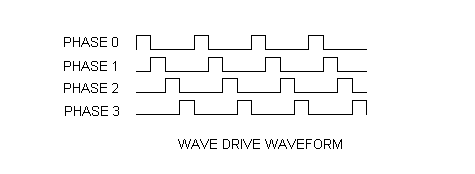
\includegraphics[width=0.6\textwidth]{figures/image50.png}
\captionsetup{type=figure}
\captionof{figure}{Fasi per pilotaggio stepper unipolare}
\end{center}

\begin{center}
\includegraphics[width=0.9\textwidth]{figures/image44.png}
\captionsetup{type=figure}
\captionof{figure}{Output SALMO su oscilloscopio}
\end{center}

\hypertarget{funzionamento-generale-del-codice}{%
\section{Funzionamento generale del
codice}\label{funzionamento-generale-del-codice}}

\begin{center}
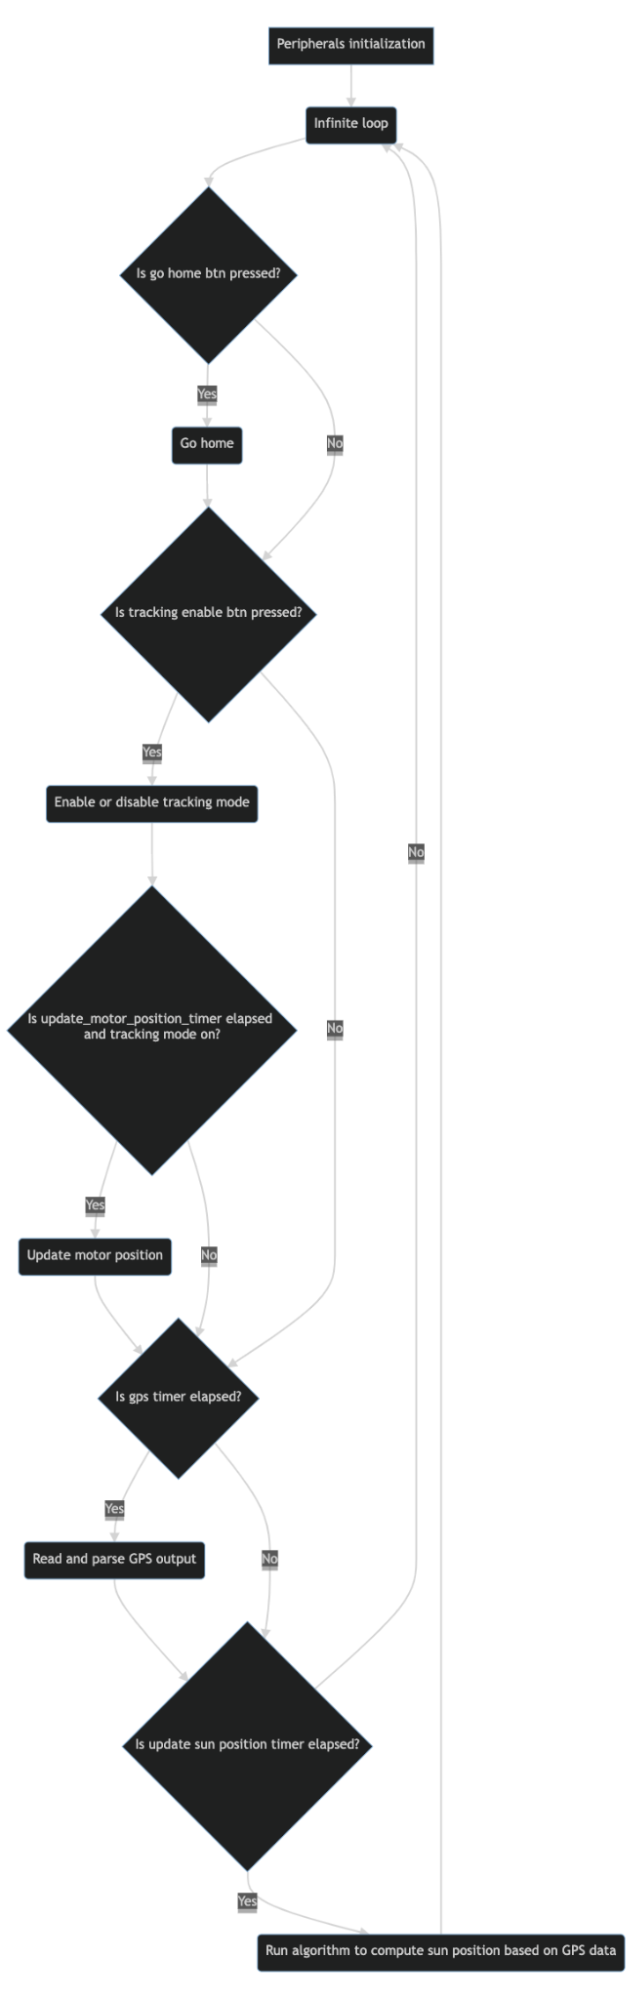
\includegraphics[width=0.43\textwidth]{figures/image36.png}
\captionsetup{type=figure}
\captionof{figure}{Flowchart del funzionamento del codice}
\end{center}

\noindent Come prima cosa vengono inizializzate le varie periferiche e moduli
ovvero:

\begin{itemize}
\item
  
  UART
  
\item
  
  USB CDC
  
\item
  
  I2C
  
\item
  
  Accelerometro
  
\item
  
  Magnetometro
  
\item
  
  Motore stepper
  
\end{itemize}

\noindent Dopodiché il microcontrollore entra in loop infinito in cui vengono
controllati degli input e delle variabili interne impostate dai timer.
Sono presenti tre timer che scandiscono:

\begin{itemize}
\item
  
  Lettura input gps (ogni 4 secondi)
  
\item
  
  Aggiornamento della posizione del motore (ogni 10 secondi)
  
\item
  
  Aggiornamento posizione del sole mediante algoritmo (ogni 4 secondi)
  
\end{itemize}

\noindent Entrati nel loop infinito viene controllato, tramite interrupt, se il
pulsante di \emph{``Go home''} (\emph{SW3}) viene premuto; qualora
succeda, i motori vengono azionati per dirigere il pannello verso il
\emph{Nord} ottenuto dalla bussola ed a 45° di elevazione (tilt).
Successivamente viene verificato, sempre tramite interrupt, se il
pulsante di ``Tracking enable/disable'' (\emph{SW4}) viene premuto. In
questo caso il flag di tracking viene abilitato o disabilitato in base
al numero di iterazioni col pulsante, infatti ad ogni pressione il flag
viene negato, pertanto dopo averlo premuto una volta il motore rimarrà
in tracking mode e se il pulsante verrà azionato di nuovo il flag di
tracking verrà disabilitato. Alla scadenza del timer relativo al
tracking, se il flag dovuto al pulsante è abilitato, viene aggiornata la
posizione del motore. Dopodichè viene controllato se il timer relativo
alla lettura del gps è terminato, in caso affermativo viene eseguita la
lettura via \textit{UART} ed il relativo parsing. Infine viene controllato se il
timer relativo alla posizione del sole è scaduto, e di conseguenza viene
o meno eseguito il calcolo della posizione del sole basandosi sui dati
ottenuti dal GPS. Il programma poi ritorna nel loop principale e
continua il controllo delle variabili.\\
A causa della mancanza di accelerometro, pannello e struttura di
supporto per i motori, ulteriori \emph{feature} verranno implementate in
futuro.